\chapter{Rio Bus}\label{chp:CAP_RIOBUS}

Uma aplicação real que faz uso dos DAGs e que serviu como plataforma para este trabalho é o \textbf{Rio Bus}\cite{riobus_sc}, projeto do qual faço parte. Criado por alunos do curso de Bacharelado em Ciência da Computação da UFRJ, o Rio Bus surgiu em 2014 como um aplicativo para visualizar em um mapa a posição em tempo real dos ônibus municipais do Rio de Janeiro, utilizando os recém-lançados dados abertos de mobilidade oferecidos pela Prefeitura do Rio de Janeiro. Com esse serviço, o cidadão pode estimar o quanto vai demorar para seu ônibus chegar e, assim, se planejar melhor.


\begin{figure}
  \centering
  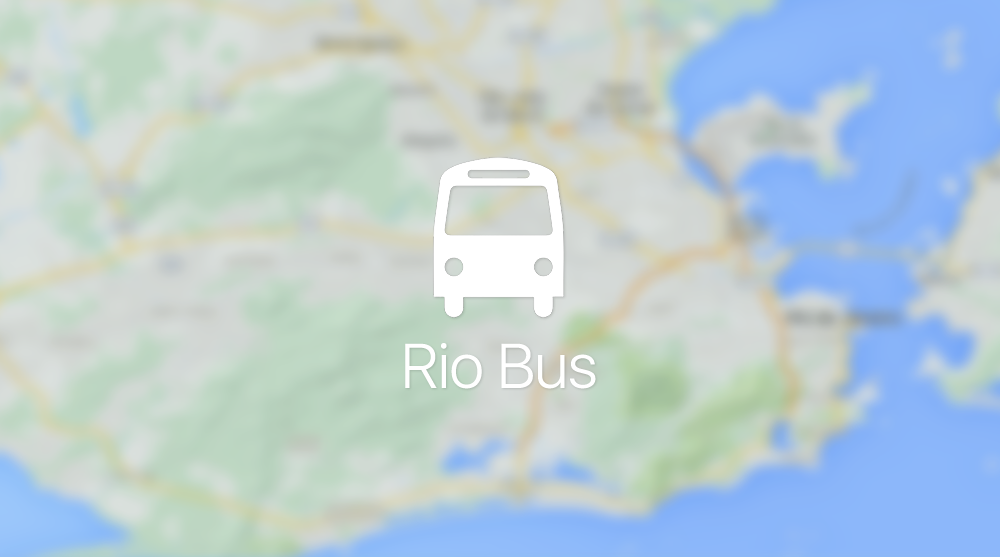
\includegraphics[width=0.5\textwidth]{imagens/riobus.png}
  \label{fig:LABEL_FIG_RIOBUS}
\end{figure}


Lançado gratuitamente e como um projeto de \textit{open-source}, o Rio Bus logo conseguiu vários colaboradores, usuários do aplicativo, dentro da UFRJ, haja vista a grande demanda por transporte público no campus da Universidade. A solução foi então disponibilizada em diferentes plataformas - um \textit{website}, disponível em \cite{REF_RIOBUS_WEB}, para acesso pelo computador ou dispositivos móveis, e dois aplicativos para \textit{smartphones}, um para o sistema operacional \textit{Android}, do Google, disponível em \cite{REF_RIOBUS_ANDROID}, e outro para \textit{iOS}, da Apple, disponível em \cite{REF_RIOBUS_IOS}.

Pouco tempo após seu lançamento, o aplicativo ganhou uma grande repercussão e serviu como ferramenta para muitos cidadãos durante a greve dos ônibus, em março de 2014. Durante a paralisação, na qual cerca de 80\% da frota de ônibus do município não saiu da garagem das empresas, muitos usuários fizeram uso do aplicativo para saber se suas linhas de ônibus estavam circulando e acompanhar onde estavam os coletivos. Esse evento não só serviu como a tração que o Rio Bus precisava para seu sucesso, como também foi um grande \textit{insight} de que coletar os dados que vinham sobre os ônibus poderia servir para uma análise do funcionamento do serviço. Esses estudos não só ajudaram a melhor compreender o serviço dos ônibus no Rio e suas falhas, como também podem ter importância especial durante períodos atípicos como paralisações, alterações no sistema, grandes eventos e ocorrências de trânsito na cidade.


\section{Base de dados}

\subsection{Origem}

Para popular a base de dados do Rio Bus, são utilizados os dados dos ônibus fornecidos pelo Data.rio\cite{data.rio}, o portal de dados abertos da Prefeitura do Rio de Janeiro. O Data.rio disponibiliza um total de 1200\footnote{Número de conjuntos de dados disponíveis em http://data.rio/ em 6 de julho de 2016} conjuntos de dados (\textit{datasets}) que estão classificados em 13 grupos - entre eles, Urbanismo, Administração Pública, Impostos e Transporte e Mobilidade, que foi o grupo utilizado.

Dentre os dados de Transporte e Mobilidade, há 23 conjuntos de dados que incluem informações sobre ônibus, trens, metrô, barcas e bicicletários do Rio de Janeiro. Estamos interessados em 3 desses \textit{datasets}: GPS dos ônibus, Pontos de parada das linhas do ônibus e Pontos dos trajetos das linhas de ônibus. Esses dados são fornecidos em parceria da Prefeitura do Rio com a FETRANSPOR (Federação das Empresas de Transporte de Passageiros do Estado do Rio de Janeiro).


\subsection{Formatos}

São utilizados diferentes formatos para acesso aos dados do Data.rio. Os dados dos pontos de parada e pontos de trajeto das linhas dos ônibus são dados tipicamente estáticos - isto é, não costumam sofrer alterações frequentes - e são disponibilizados em uma planilha em formato CSV (Comma-separated values). Eles são atualizados com baixa frequência na base de dados do Rio Bus.

Já os dados de GPS dos ônibus, como são atualizados diversas vezes por minuto, podem ser acessados através de uma API (Application Programming Interface) que retorna um objeto JSON (JavaScript Object Notation) contendo os dados de cada ônibus naquele instante. Esses dados são coletados com alta frequência para popular a base de dados do Rio Bus, formando assim uma coleção histórica dos dados. Um exemplo de como se parece essa coleção está na tabela \ref{table:collection_bus}, que mostra um trecho dos registros de um ônibus da linha 325 no dia 09/07/2015.

\begin{table}[]
\centering
\caption{Exemplo da coleção histórica de um ônibus}
\label{table:collection_bus}
\begin{tabular}{|p{2.5cm}|c|c|c|c|c|c|}
\hline
\multicolumn{7}{|c|}{\textbf{Trecho da coleção histórica do ônibus B28518 da linha 325}} \\
\hline
\textbf{Data/hora} & \textbf{Ordem} & \textbf{Linha} & \textbf{Lat.} & \textbf{Long.} & \textbf{Veloc
.} & \textbf{Direção} \\ \hline
09/07/2015 23:19:05 & B28518 & 325 & -22.815200 & -43.188300 & 41 & 306\\\hline
09/07/2015 23:20:18 & B28518 & 325 & -22.815700 & -43.188100 & 20 & 165\\\hline
09/07/2015 23:21:35 & B28518 & 325 & -22.815700 & -43.188000 & 37 & 150\\\hline
\end{tabular}
\end{table}


\subsection{Armazenamento}

Como o volume de dados proveniente da atualização dos ônibus é muito grande, as APIs do Data.rio fornecem apenas os dados do instante atual. Para que pudéssemos ter acesso aos dados de períodos passados, utilizamos a infraestrutura do \textit{back-end} do Rio Bus para armazenar esses dados, que ultrapassam 9 milhões de novos registros por dia.

Para isso, temos um serviço que executa indefinidamente que faz a leitura dos dados do Data.rio e os salva num banco de dados próprio. Na implementação atual, os dados são salvos em dois lugares: numa coleção do MongoDB, um banco de dados não-relacional open-source instalado localmente, e no Google BigQuery, um serviço de cloud para armazenamento e análise de dados em larga escala (\textit{Big Data}), como é o nosso caso.

Para os propósitos deste trabalho, daremos preferência ao banco de dados MongoDB\cite{REF_MONGODB} para executar as consultas. Ainda que a implementação das consultas nele seja mais difícil - o Google BigQuery\cite{REF_BIGQUERY} suporta consultas com SQL - a decisão leva em conta o acesso à informação - o BigQuery é um serviço pago, remoto e de código fechado, enquanto o MongoDB é uma aplicação que pode ser executada localmente, sem custos e que possui o código aberto, de acordo com os princípios deste projeto.
